% mnras_template.tex 
%
% LaTeX template for creating an MNRAS paper
%
% v3.0 released 14 May 2015
% (version numbers match those of mnras.cls)
%
% Copyright (C) Royal Astronomical Society 2015
% Authors:
% Keith T. Smith (Royal Astronomical Society)

% Change log
%
% v3.0 May 2015
%    Renamed to match the new package name
%    Version number matches mnras.cls
%    A few minor tweaks to wording
% v1.0 September 2013
%    Beta testing only - never publicly released
%    First version: a simple (ish) template for creating an MNRAS paper

%%%%%%%%%%%%%%%%%%%%%%%%%%%%%%%%%%%%%%%%%%%%%%%%%%
% Basic setup. Most papers should leave these options alone.
\documentclass[fleqn,
%referee, % this line changes to double-spaced 1 column
usenatbib]{mnras}


% MNRAS is set in Times font. If you don't have this installed (most LaTeX
% installations will be fine) or prefer the old Computer Modern fonts, comment
% out the following line
\usepackage{newtxtext,newtxmath}
\usepackage{anyfontsize}
% Depending on your LaTeX fonts installation, you might get better results with one of these:
%\usepackage{mathptmx}
%\usepackage{txfonts}

% Use vector fonts, so it zooms properly in on-screen viewing software
% Don't change these lines unless you know what you are doing
\usepackage[T1]{fontenc}

% Allow "Thomas van Noord" and "Simon de Laguarde" and alike to be sorted by "N" and "L" etc. in the bibliography.
% Write the name in the bibliography as "\VAN{Noord}{Van}{van} Noord, Thomas"


%%%%% AUTHORS - PLACE YOUR OWN PACKAGES HERE %%%%%

% Only include extra packages if you really need them. Common packages are:
\usepackage{graphicx}	% Including figure files
\usepackage{amsmath}	% Advanced maths commands
% \usepackage{amssymb}	% Extra maths symbols
\usepackage{hyperref}
\usepackage[normalem]{ulem}
\usepackage[dvipsnames]{xcolor}
% \usepackage{enumitem}

\graphicspath{{figures/}} 
% \linespread{1.8}




%%%%%%%%%%%%%%%%%%%%%%%%%%%%%%%%%%%%%%%%%%%%%%%%%%

%%%%% AUTHORS - PLACE YOUR OWN COMMANDS HERE %%%%%

% Please keep new commands to a minimum, and use \newcommand not \def to avoid
% overwriting existing commands. Example:
%\newcommand{\pcm}{\,cm$^{-2}$}	% per cm-squared


% citations
\defcitealias{james+21}{J21}
\newcommand{\JJ}{\citetalias{james+21}}
\newcommand{\VICE}{\textsc{vice}}

\newcommand{\citetjack}{\citet{jack}}
\newcommand{\citepjack}{(Roberts et al.~2024, in prep.)}
\newcommand{\citealtjack}{Robert et al.~2024, in prep.}
\newcommand{\cxi}{\texttt{\hyperlink{C11}{C11}}}
\newcommand{\pxvi}{\texttt{\hyperlink{P16}{P16}}}
\newcommand{\kxvi}{\texttt{\hyperlink{K16}{K16}}}
\newcommand{\vxiii}{\texttt{\hyperlink{V13}{V13}}}
\newcommand{\cfactor}{2.4}
\newcommand{\nsubgiants}{16,365}



% Acronyms
\newcommand{\agb}{AGB}
\newcommand{\apogee}{APOGEE}
\newcommand{\aspcap}{\textsc{aspcap}}
\newcommand{\cc}{CCSN}
\newcommand{\gce}{GCE}
\newcommand{\ia}{SN Ia}

% internal abbreviations
\newcommand{\caah}{[C/Mg]-[Mg/H]}
\newcommand{\caafe}{[C/Mg]-[Mg/Fe]}


% other
\newcommand{\ycmg}{\ensuremath{2.7 + 32\left(Z-\Zo\right)}}
\newcommand{\ycccmg}{1}
\newcommand{\yco}{1}
\newcommand{\fmeas}{20\%}

\makeatletter
\newcommand{\C}[1][\@nil]{
    \def\tmp{#1}%
    \ifx\tmp\@nnil%
        \ensuremath{\rm C}%
    \else%
        \ifmmode ^{#1}{\rm C}%
        \else $^{#1}$C%
        \fi%
\fi }
\makeatother

\newcommand{\Yct}{\ensuremath{y_{\rm C}}}
\newcommand{\Ycc}{\ensuremath{y_{\rm C}^{\rm CC}}}
\newcommand{\Yoc}{\ensuremath{y_{\rm Mg}^{\rm CC}}}
\newcommand{\Ycagb}{\ensuremath{y_{\rm C}^{\rm AGB}}}
% \newcommand{\y}{\ensuremath{\rotatebox[origin=B,y=0.5ex]{180}{y}}}
\newcommand{\y}{Y}

\newcommand{\Mo}{%
    \ifmmode {\rm M}_{\sun}%
    \else {M$_{\sun}$}%
    \fi}
    
\newcommand{\Zo}{%
    \ifmmode Z_{\sun}%
    \else $Z_{\sun}$%
    \fi}

\newcommand{\about}[1]{${\sim} #1$}

%%% citepos command
\makeatletter
\DeclareRobustCommand\citepos
  {\begingroup
   \let\NAT@nmfmt\NAT@posfmt% ...except with a different name format
   \NAT@swafalse\let\NAT@ctype\z@\NAT@partrue
   \@ifstar{\NAT@fulltrue\NAT@citetp}{\NAT@fullfalse\NAT@citetp}}

\let\NAT@orig@nmfmt\NAT@nmfmt
\def\NAT@posfmt#1{\NAT@orig@nmfmt{#1's}}

\makeatother


%%%%%%%%%%% JWJ' editing macros %%%%%%%%%%%
\newcommand{\strike}[1]{{\color{ForestGreen} \sout{#1}}}
\newcommand{\add}[1]{{\color{ForestGreen} #1}}
\newcommand{\note}[1]{{\color{ForestGreen} \textit{ \small (JWJ: #1)}}}
% \LetLtxMacro\origcitep\citep
% \LetLtxMacro\origcitet\citet
% \renewcommand{\citep}[2][]{%
%     \mbox{\origcitep[#1][]{#2}}
% }
% \renewcommand{\citet}[2][]{%
%     \mbox{\origcitet[#1][]{#2}}
% }

\newcommand{\dbstrike}[1]{{\color{Thistle} \sout{#1}}}
\newcommand{\dbadd}[1]{{\color{Thistle} #1}}
\newcommand{\dbnote}[1]{{\color{Thistle} \textit{\small (DB: #1)}}}


% \LetLtxMacro\origcite\cite

% This is my command. I want to strike out, 
% \newcommand{\strikeit}[1]{%
%   \ifcorrectingmode
%   \mbox{\sout{#1}}%
% %  \makebox[\textwidth][s]{\sout{#1}}%
%   \fi
% }

% \renewcommand{\cite}[2][]{%
%   \ifcorrectingmode
%   \mbox{\origcite[#1]{#2}}%
%   \else
%   \origcite[#1]{#2}%
%   \fi
% }




%%%%%%%%%%%%%%%%%%%%%%%%%%%%%%%%%%%%%%%%%%%%%%%%%%

%%%%%%%%%%%%%%%%%%% TITLE PAGE %%%%%%%%%%%%%%%%%%%

% Title of the paper, and the short title which is used in the headers.
% Keep the title short and informative.
\title[The Origin and Galactic Evolution of Carbon]{The Galactic Chemical Evolution of Carbon: Implications for Stellar Nucleosynthesis }

% The list of authors, and the short list which is used in the headers.
% If you need two or more lines of authors, add an extra line using \newauthor
\author[D. A. Boyea et. al.]{%
Daniel A. Boyea,$^{1, 2, 3}$\thanks{%
Contact e-mail:~\href{mailto:boyea.2@osu.edu}{boyea.2@osu.edu}}
James W. Johnson,$^{1, 2, 4}$
Third Author$^{2,3}$
and Others$^{1,3}$
\\
% List of institutions
$^{1}$Department of Astronomy, The Ohio State University, 140 W. 18th Ave., Columbus, OH, 43210, USA
\\
$^{2}$Center for Cosmology \& Astroparticle Physics (CCAPP), The Ohio State University, 191 W. Woodruff Ave., Columbus, OH, 43210, USA
\\
$^{3}$Department of Physics \& Astronomy, University of Victoria, Victoria, BC V8P 5C2, Canada
\\
$^{4}$The Observatories of the Carnegie Institution for Science, 813 Santa Barbara St., Pasadena, CA, 91101, USA
}

% These dates will be filled out by the publisher
\date{Accepted XXX. Received YYY; in original form ZZZ}

% Enter the current year, for the copyright statements etc.
\pubyear{2024}

% Don't change these lines
\begin{document}
\label{firstpage}
\pagerange{\pageref{firstpage}--\pageref{lastpage}}
\maketitle



% Abstract of the paper
\begin{abstract}
% context
The origin of C, despite its importance, remains poorly understood. 
% 
We aim to constrain the stellar yields of C through multi-zone Galactic chemical evolution models by comparing predictions with \apogee\ subgiants abundances.
% 
We find that \caafe\ trends, when restricted in metallicity, are an empirical estimate of the delayed C sources, enabling us to estimate that \agb\ stars and \cc\ produce about 20\% and 80\% of C, respectively.  
The \caah\ trend instead represents the equilibrium abundances of C and Mg. 
We use the \caah\ trend to estimate the CCSNe C/Mg yield, determining that  $\Ycc/\Yoc = EQUATION$ when including \agb\ C. 
% misc
Our models are relatively independent of uniform scaling of yields and outflows, and alternate star formation histories. 
However, the stars which contribute to \agb\ C production and the \ia\ delay time distribution of Fe contribute uncertainties to our conclusions. 
% gas phase
While reliable gas-phase and low-metallicity measurements of C are challenging, we find that our model and a single-zone model with our recommended yields replicate the broad trends of \caah{} across different environments and metallicities. 

\end{abstract}

\begin{keywords}
galaxies: abundances -- galaxies: evolution -- galaxies: star formation -- galaxies: stellar content -- methods: numerical
\end{keywords}



%%%%%%%%%%%%%%%%%%%%%%%%%%%%%%%%%%%%%%%%%%%%%%%%%%

%%%%%%%%%%%%%%%%% BODY OF PAPER %%%%%%%%%%%%%%%%%%

\section{Introduction}

Despite being one of the most abundant metals in the universe~\citep[e.g.][]{asplund+09}, C nucleosynthesis is poorly understood.
Formed in the cores of stars during He fusion, C is the first \dbadd{primary? element} after He. Additionally, C is one of the only light elements formed in low-mass stars \citep[e.g.,][]{KL14}. \dbnote{I don't like how many e.g.'s there are, and is this the right citation here?}
\dbadd{
Because the effects of first dredge up are mass-dependent, C and N abundances are frequently used as age indicators for RGB stars \citep{MG15, martig16, hasselquist19, vincenzo+21}. 
}
\dbnote{C abundnces for stellar structure (opacities) and star formation (line cooling)}
Broadly, it is well understood that both lower-intermediate-mass and high-mass stars produce C. However, the relative yields from these two classes of stars and their dependence on  metallicitys unknown \add{(see discussion below)}.

% \footnotetext{\strike{By metallicity, we mean the (mass) fraction of any element which is not H or He, denoted by $Z$. For the sun, we take $Z_\odot=0.016$. CHECK THIS~} }



Like many other metals, C nucleosynthesis \dbstrike{is poorly understood because its predicted yields} \dbadd{predictions from stellar evolution are highly uncertain \citep[see reviews][]{romano+10, KL14}}.
\strike{Yield predictions} are shaped by poorly understood processes, such as mass loss rates \citep{ventura+13}?, nuclear reaction networks, rotational mixing \citep{frischknecht+16, LC18}, and convection ~\citep{chieffi2001}. \dbnote{check citations here...}. 
Binarity (and the metallicity dependence thereof), e.g. MKB2019, farme,
Small changes in the initial mass ($0.01\Mo$) of massive stars can dramatically change the subsequent evolution \citep{bruenn+2023, emily+21}. As such, accurate yield predictions would require a much more densly sampled set of models in mass, metallicity, and rotation rates then are presently available. Furthermore, binary evolution is rarely included in massive star models with possibly important implications for yields \citep{farmer+21}, despite the large (metallicity-dependent) fraction of massive stars which live in binary systems \citep{MKB2019}.

\dbnote{added paragraph here}
In light of these difficulties with accurate theoretical modeling, recent work has instead sought to characterize chemical yields empirically.
\citet{HLA20} measured the abundance ratios in the ejecta of Cassiopeia A using spatial resolved X-ray spectra.
\citet{weinberg+19, weinberg+22} analyzed the abundance ratio trends of high- and low-alpha sequence stars in APOGEE~\citep{apogee17} to infer relative yields of prompt and delayed enrichment sources and the metallicity dependence thereof.
\citet{emily+19, emily+22, emily+23} applied the same methodology to GALAH~\citep{DeSilva2015, Martell2017}.
\citet{rodriguez+21, rodriguez+23} measured the mean Fe yield of core-collapse supernovae (CCSNe) using the radioactive tails of their lightcurves.


\dbnote{combine this with previous, shorten J23 description and call out other ongoing work e.g. Miquela's He, James's chemical equilibrium, ...}
Most notably for our purposes,~\citet{james+23} used Galactic chemical evolution (GCE) models to show that the correlation between gas-phase N and O abundances (see their Fig. 1) can be explained by the metallicity dependence of relative N and O yields. 
Variations in assumptions regarding GCE parameters, such as the detailed star formation history (SFH), did not impact their conclusions and are instead a likely source of scatter in the observed relation.
Here, we apply similar methodology to constrain C yields, which are closely related to N.




GCE connects a galaxy's evolutionary history to the detailed elemental abundances in its gas and stars.
Each enrichment process has characteristic chemical signatures and timescales, enabling us to reconstruct \strike{chemical} \add{enrichment} histories.
\add{As an element that is well-measured in stellar spectra, many} \dbadd{with large samples of stellar C abundancess}, \strike{Many} previous GCE works \add{have} focused on C abundances (\citealt{DTS78, BF06, prantzos+18, berg+19}; see also the recent reviews by \citealt{romano22} and \citealt{RM21}).
To date there is no consensus on the detailed origin of C; some authors have argued that high-mass stars should dominate~\citep[e.g.][]{prantzos+94, HEK00, romano+20, franchini+20, gustafsson22}, and others have argued that AGB stars should contribute at least half of the C in the universe~\citep[e.g.][]{tinsley79, chiappini+03, mattsson10, KKU11, rybizki+17, KKL20}. 

    As our primary observational constraint, we use a sample of subgiant stars from the \apogee{} \citep{apogee17} selected by the criteria in \citetjack.
According to stellar evolution theory and observations, subgiants most accurately represent their birth composition \citep{gilroy89, korn+07, lind+08, souto+18, souto19}.
Fig.~\ref{fig:subgiants} shows the subgiant sample plotted in \caah\ and \caafe{}.\footnotemark{} In this sample, [C/Mg] increases with metallicity, and [C/Mg] decreases with [Mg/Fe] at fixed [Mg/H]. 
From observations of nearby stars and (extragalactic) gas, we know that [C/O] against [O/H] traces a banana shape (see Fig.~\ref{fig:gas_phase} and section~\ref{sec:gas}).
At the very lowest metallicities\strike{, where} \add{(}$[{\rm O/H}]\lesssim-2$\add{)},%
%
observations \strike{suggest} \add{indicate} that [C/Mg] declines with metallicity.
From $-2 \lesssim {\rm [O/H]}\lesssim -1$, [C/Mg] is roughly constant with metallicity. 
At higher metallicities ([O/H]~$\gtrsim -1$), [C/Mg] increases with metallicity.

\strike{Using the subgiant abundance trends, we will develop a model of the enrichment sources and evolution of C.}
\add{We will show in section~\ref{sec:results} below that these correlations in the bulk population abundances alone are quite constraining for the origin of C.}

\footnotetext{In this paper, we use the standard notation for chemical abundances. $[A/B] = \log_{10}\left(A/B\right) - \log_{10}\left(A_{\sun}/B_{\sun}\right)$, i.e. $[A/B]$ is the logarithm of the mass ratio between A and B, scaled such that $[A/B]=0$ for the sun (see Table~\ref{tab:fiducial_mod} for solar scale.)}


In Section~\ref{sec:data_selection} we describe the selection for our subgiant observational sample.
Section~\ref{sec:nucleosynthesis} discusses theoretical estimates of \agb\ and \cc\ C yields. We parameterize our yield choices and derive a estimate of C/Mg yields observationally.
Section~\ref{sec:vice} reviews the multizone model and modifications thereof for this work.
Section~\ref{sec:results} presents our multizone model predictions and GCE parameters which are observationally permissable. 
Finally Section~\ref{sec:gas} compares our model to literature collected observations of halo stars and extragalactic HII regions. 





\section{Data Selection}\label{sec:data_selection}


\begin{figure*}
    \centering
    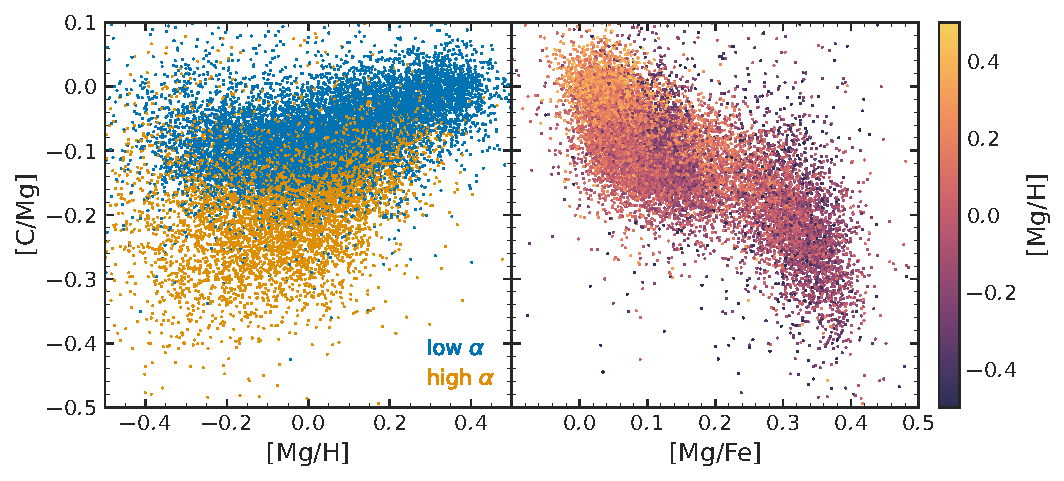
\includegraphics{subgiants.pdf}
    \caption{The [C/Mg] ratio against [Mg/H] (top) and [Mg/Fe] (bottom) for the \citetjack~sample of \apogee{} subgiants. On the top, we plot high and low-$\alpha$ stars in blue and orange, using the separation defined in Equation \ref{eq:high_alpha} (the high and low-$\alpha$ stars are named for their high or low $\alpha$-element to Fe ratios, or in this case, Mg/Fe). On the bottom, we colour-code stars according to their [Mg/H] abundance.} \label{fig:subgiants}
\end{figure*}


% Subgiants are a useful empirical benchmark because their photospheric abundances should reflect their birth mixture. 
As an emperical benchmark, we use subgiant stars, whose photospheres accurately represent birth abundances. 
During main sequence evolution, metals can fall to below the convective envelope (i.e., ``gravitational settling").
When stars leave the main sequence and become subgiants, these metals are mixed with the convective envelope \citep[]{gratton+00, souto19}. 
 \textit{First dredge up} during the red giant phase brings CNO processed core material to the surface \citet{iben67, KL14}.
 
We use the sample of \apogee\ DR17 subgiants from \citetjack, selecting stars within the $\log g$-$T_\text{eff}$ polygon given by
 \begin{equation}
    \begin{cases} \label{eq:subgiant_selection}
        \log \text{g} \geq 3.5 \\
        \log \text{g} \leq 0.004\,T_{\rm eff} - 15.7 \\
        \log \text{g} \leq 0.000706\,T_{\rm eff} + 0.36 \\
        \log \text{g} \leq -0.0015\,T_{\rm eff} + 12.05 \\
        \log \text{g} \geq 0.0012\,T_{\rm eff} - 2.8. \\
    \end{cases}
\end{equation}
Also following \citet{jack}, we exclude stars with the flags:
        \verb|APOGEE_MIRCLUSTER_STAR|,
        \verb|APOGEE_EMISSION_STAR|,
        \verb|APOGEE_EMBEDDEDCLUSTER_STAR|,
        \verb|APOGEE2_YOUNG_CLUSTER|,
            \verb|APOGEE2_W345|,
        \verb|APOGEE2_EB|, and
        \verb|ASPCAP_BAD|.
We additionally remove stars with no reported C, Mg, or Fe abundances. These cuts yield a sample containing \nsubgiants\ subgiants.




\section{Nucleosynthesis}\label{sec:nucleosynthesis}


Table \ref{tab:fiducial_mod} contains our fiducial yields and abundance scale. 
For O, Mg, and Fe, we adopt the yields in \citet{david_fe}. We use a scaled variation of the N yield from \citet{james+23}. 
Following \citet{james+21, james+23}, we take the \ia{} delay time distribution to be a $t^{-1.1}$ power-law with a minimum delay time of 150\,Myr, as suggested by the observations of \citet{maoz+12}. We use solar abundances from \citet{magg+22} with a +0.04 gravitational settiling correction as in \citet{david_fe}. \dbadd{Magg22 finds Z/X = 0.0225 for the surface? what do we use for the solar metallicity?}. Assuming He abundance from $Y=0.2725$ from \citet{AAG2021}, resulting in a $Z_\odot=0.01606$


\begin{table}
	\centering
    \caption[]{Solar abundance scale and fiducial yields (in units of SSP~birth mass). See section \ref{sec:agb} for the definition of \cxi. The solar abundance scale is \citet{magg+22} + 0.04. }
	\label{tab:fiducial_mod}

	\begin{tabular}{l l l l l}
		\hline
        Element & $Z_{X,\,\sun}$ & $y_X^{\rm cc}$ & $\y_X^{\rm agb}$ & $y_X^{\rm ia}$  \\
		\hline
        C & 0.00339 & Eq.~\ref{eq:y_cc} & $\cfactor\times$\cxi &  0 \\
        O & 0.00733 & 7.12e-3 & 0 & 0 \\
        Mg & 0.000671 & 6.69e-4 & 0 & 0 \\
        Fe & 0.00137 & 4.72e-4 & 0 & 6.69e-4 \\
        N &0.00104 & 4.001e-4 & 0.0009$M\left(\frac{Z}{Z_\odot}\right)$ & 0\\
        % C & 0.00339 & Eq.~\ref{eq:zeta} & $\cfactor\times$\cxi &  0 \\
        % O & 0.00733 & 0.015 & 0 & 0 \\
        % Mg & 0.000671 & 0.00185 & 0 & 0 \\
        % Fe & 0.00137 & 0.0012 & 0 & 0.00214 \\
        % N &0.00104 & 0.00072 & 0.0009$M\left(\frac{Z}{Z_\odot}\right)$ & 0\\
		\hline
	\end{tabular}
\end{table}


\dbnote{I like the definition of Y to go here since that is model independent, but IMF-integrated could still be specific to AGB/CC.}


\subsection{Asymptotic Giant Branch Stars}\label{sec:agb}

An Asymptotic Giant Branch (AGB) star is a low mass star during its last nuclear burning phase (He shell burning; see e.g. \citealt{PR2023}) which enriches the ISM through mass loss during thermal pulses.
    In this work, we explore four different stellar AGB yield tables from the literature which provide
    well-sampled grids in mass and metallicity. We refer to the tables as 
\begin{description}
    \item \hypertarget{C11}{\texttt{C11}}: \citet{cristallo+11, cristallo+15}
    \item \hypertarget{V13}{\texttt{V13}}: \citet{ventura+13,ventura+14,ventura+18, ventura+20}
    \item \hypertarget{K16}{\texttt{K16}}: \citet{KL16, karakas+18}
    \item \hypertarget{P16}{\texttt{P16}}: \citet{pignatari+16, ritter+18, battino+19, battino+21}
\end{description}
Table~\ref{tab:agb} notes the masses and metallicities for each grid of yields.
We use the same tables as \citet{james+23}, except that we have swapped \citet{karakas10} for \citet{ritter+18}. 

We define a yield to be the fraction of a star's initial mass $M_{\rm birth}$ which is converted into freshly synthesized C. If $\Delta Z_{\rm C}$ represents the change in the mass fraction of C abundance, then
\begin{equation}
    \y_{\rm C}^{\rm AGB} =  \Delta Z_{\rm C} \frac{M_{\rm ejected}}{M_{\rm birth}}.
\end{equation}
The yields may be negative if the material returned to the ISM has a lower $Z_{\rm C}$ than the material the star was formed from.


Fig.~\ref{fig:y_agb} compares the stellar \agb\ C yields for these four models.
Most models agree on general yield trends in mass and metallicity.
C production peak between masses of $\sim$ 2--4 \Mo\ and declines as stars become more or less massive. As metallicity increases, the net yield decreases and the mass of peak C production increases slightly.



The left panel of Fig.~\ref{fig:agb-ssp} shows IMF-averaged C yields for each \agb\ model as a function of metallicity.
An IMF-averaged yield adds together the yields of stars of each mass, weighted by the fraction of stars of each mass (the IMF). 
\begin{equation} \label{eq:imf-agb-yield}
    \Ycagb(Z,\tau) = 
    \frac{
    \int_{M_{\rm to}(\tau)}^{8\,\Mo} 
    \y_{\rm X}(M, Z) M\ 
    \frac{dN}{dM}\ dM
}
{
    \int_{0.08\Mo}^{100\Mo}\ M\ \frac{dN}{dM}\ dM
}
\end{equation}
where ${dN}/{dM}$ is the IMF and $M_{\rm to}(\tau)$ is the mass of stars with lifetime $\tau$.%
\footnote{In this paper, we take the metallicity-independent parabola in $\log \tau$-$\log m$ space from \citet{larson74} as our mass-lifetime relation.} \dbnote{are the numbers in the integral bounds okay here or should we write this out or put in footnote? And should we be using a more recent MLR?}
The \agb\ models mostly differ in their yield normalization and metallicity dependence. 
The normalizations span a factor of \about{2}.
For example, at $Z = 0.1\Zo$, each models predicts $Y_{\rm C}^{\rm AGB}$ to be between 0.0008 and
0.0016.
The metallicity dependence of the yields span a factor of \about{3} (see $\zeta^{\rm AGB}$ in
Table~\ref{tab:agb} and discussion in section~\ref{sec:equilibrium} below).
Variations in \agb\ models are due to different choices of reaction rates, convection treatments, and mass-loss rates. 



The right panel of Fig.~\ref{fig:agb-ssp} shows the total production of C by \agb\ stars by a SSP as a function of age at solar metallicity. 
As the mass range $2\,\Mo\lesssim M \lesssim 4\,\Mo$ is most important for C production, half the yield is produced before \about{1}\,Gyr, similar to Fe production by \ia. 
\kxvi{} weight C production more heavily towards high-mass \agb\ stars, resulting in shorter delay times, whereas the \cxi\ and \vxiii\ models predict a slightly longer timescale of \about{1}\,Gyr. In any case, little to no C is produced more than 2\,Gyr after a star formation event. Fe production, in contrast, continues steadily for 10\,Gyr. 

In \agb\ stars, two competing processes determine the outcome of C production: {third dredge up} (TDU) and {hot bottom burning} (HBB).  
TDU accompanies thermal pulses in \agb\ stars, where material from the CO core is mixed with the envelope, increasing surface C abundances \citep{KL14}. The C yields of the star are increased as this C-enhanced envelope is released to the ISM. 
HBB\ is the activation of the CNO cycle at the bottom of the convective envelope. 
TDU increases C yields and HBB converts C into N. When both processes activate, highly efficient N production ensues (see discussion in e.g. \citealt{james+23, ventura+13}). 
%Because the $^{14}$N proton capture is the slowest component of the CNO cycle, the CNO cycle converts nearly all \C[12] into $^{14}$N \citep{solar-fusion}.

% \footnotetext{
%     The CNO cycle is a series of proton-capture reactions with CNO elements resulting in energy generation and the creation of an $\alpha$ particle. $\C[12]({\rm p}, \gamma)
%     ^{13}{\rm N}(\beta^+, \nu_{\rm e})
%     ^{13}{\rm C}({\rm p}, \gamma)\allowbreak
%     ^{14}{\rm N}({\rm p}, \gamma)\allowbreak
%     ^{15}{\rm O}(\beta^+, \nu_{\rm e})\allowbreak
%     ^{15}{\rm N}({\rm p}, \alpha)
%     \C[12]$. 
% There are other less important minor branches of the CNO cycle
%  \citep{solar-fusion}.
% }


Both HBB and TDU result in mass and metallicity dependent C yields. 
Stars less than \about{2}\,\Mo\ do not experience TDU As a result, these stars C abundances are only affected by first dredge-up (CITE), resulting in small net C yields.
Above \about{2}\,\Mo{}, TDU becomes important, enriching the outer layers with C.
In \agb\ stars more massive than \about{5}\,\Mo, efficient HBB turns most \C[12] into $^{14}$N.
Metal poor stars dredge up more material \dbnote{for which physics, compactness, mixing efficiency( Boothroyd \& Sackmann 1988))? etc.}, resulting in elevated C production \citep{ventura+13}.

For our models to better match observations, we uniformly amplify the yield tables according to
\begin{equation} \label{eq:alpha}
        \Ycagb \rightarrow \alpha_{\rm agb}\ \Ycagb.
\end{equation}
We use the \cxi\ table, with $\alpha_{\rm agb}=\cfactor$, as the fiducial \agb\ yield.


\begin{table*}
	\centering
    \caption[]{For each \agb\ yield set, the IMF-averaged \agb\ C yield at solar metallicity $y_{\rm C, 0}^{\rm agb}$ and the multiplicative factor reaches an \agb\ contribution of 20\% $\alpha_{0.2}^{\rm agb}$.}

	\label{tab:agb}
    \begin{tabular}{c cc cc  c p{5cm} p{5cm}} % four columns, alignment for each
		\hline 
        \agb\ table 
                & $y_{\rm C}^{\rm agb}(\Zo)$ & y & $\zeta^{\rm agb}(\Zo)$ & $\zeta$ &  $\alpha_{0.2}^{\rm agb}$
                & masses (\Mo) & metallicites ($\log Z/\Zo$)\\
        \hline
        \cxi 
                &  $3.5^{+0.3}_{-0.3}$ & 4.0
                & $-3.5^{+0.3}_{-0.3}$ & -3.5
                & 1.32
                & 1.3, 1.5, 2, 2.5, 3, 4, 5, 6
                & -2.15, -1.67, -1.15, -0.85, -0.67, -0.37, -0.24, -0.15, 0.0, 0.15
                \\
        \vxiii 
                & $2.7^{+1.3}_{-1.3}$ & 2.6 
                & $-4.9^{+1.4}_{-1.6}$ & -4.9
                & 2.5
                & 1.5, 2, 2.5, 3, 3.5, 4, 4.5, 5, 6, 6.5, 7
                & -1.67, -1.15, -0.85, -0.54, -0.24, 0.0, 0.46
                \\
        \kxvi 
                & $3.0^{+0.4}_{-0.5}$ & 3.5
                & $-10.1^{+0.9}_{-1.3}$ & -10
                & 1.11
                & 1, 1.25, 1.5, 1.75, 2.25, 2.5, 2.75, 3, 3.25, 3.5, 3.75, 4, 4.5, 5, 5.5, 6, 7 
                & -0.7, -0.3, 0.0, 0.33 
                \\
        \pxvi 
                & $6.2^{+1.1}_{-1.1}$ & 8
                & $-5.3^{+1.0}_{-0.9}$ & -3.
                & 1, 1.65, 2, 3, 4, 5, 6, 7
                &  -2.15 , -1.15 , -0.37 , -0.15 , 0.15
                \\
		\hline
	\end{tabular}
\end{table*}


\begin{figure*}
    \centering
 	    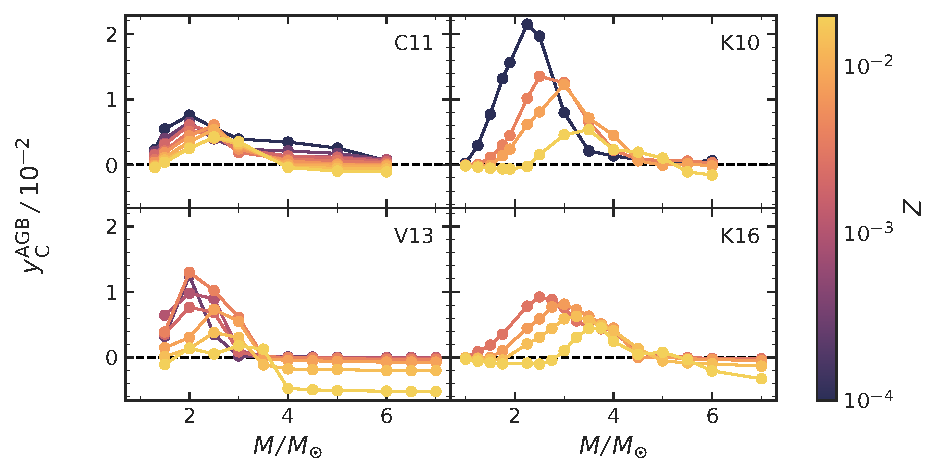
\includegraphics[scale=1]{agb_yields.pdf}
        \caption[]{The net fractional \agb\ C yield  plotted as a function of initial stellar mass $M$ and colour-coded according to metallicity. The black dashed line shows $\y=0$ for reference. Each panel represents yields from one of four \agb\ models: \cxi{}, \vxiii{}, \kxvi{}, \pxvi{} (see sections \ref{sec:agb}) }

        \label{fig:y_agb}
\end{figure*}

\begin{figure*}
    \centering
    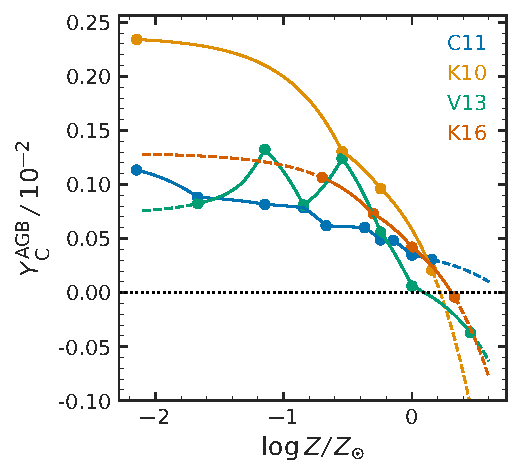
\includegraphics{y_agb_vs_z.pdf}
    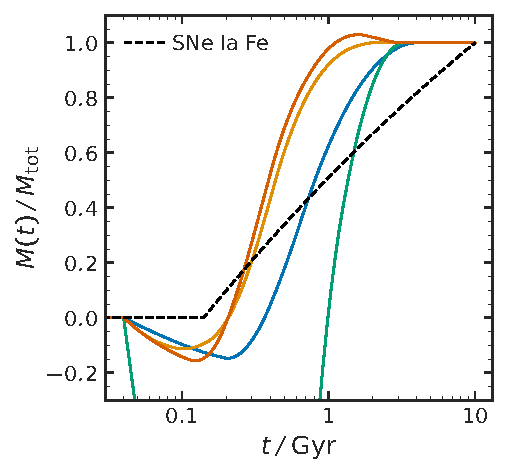
\includegraphics{y_agb_vs_t.pdf}

    \caption[]{ C yields from \agb\ stars as a function of SSP age, as a fraction of the C yield at $t_{\rm end}=10\,$Gyr. 
\textbf{Left} The (IMF-weighted) \agb\ C yield $\Ycagb$ as a function of metallicity for each of the \agb\ yield models. ($\Ycagb$ is the net mass of C produced by \agb\ stars per unit mass of star formation, after 10\,Gyr and assuming a \citealt{kroupa01} IMF.)
    \textbf{Right} Our four considered \agb\ yield models at solar metallicity (\cxi{}, \vxiii{}, \kxvi{}, \pxvi{}. The dashed red line shows the delay time distribution of type Ia supernovae ($\propto t^{-1.1}$) for comparison, and the minimum of V13 is $y(t)/y(t_{\rm end}=-46$. 
}

    \label{fig:agb-ssp}

\end{figure*}



\subsection{Core Collapse Supernovae}


Massive stars form $^{12}$C in their cores through the triple--$\alpha$ reaction.
Surviving C ejected through supernovae and winds form the massive star yields.
While there are many stellar models providing predictions of \cc{} yields, the results of these models are highly uncertain due to the complexity of stellar modeling.

Fig.~\ref{fig:y_cc} plots calculations of IMF-averaged yields for a handful of massive star yields from the literature.
For \cc\, the IMF-averaged yield is
\begin{equation} \label{eq:imf-cc-yield}
    \Ycc(Z) = 
    \frac{
    \int_{8\,\Mo}^{100\,\Mo} 
    \y_{\rm C}(M, Z)
    \frac{dN}{dM}\ M\ dM
}
{
    \int_{0.08\Mo}^{100\Mo} \frac{dN}{dM}\ M\ dM
}
\end{equation}
where ${dN}/{dM}$ is the IMF and 8\,\Mo is the assumed minimum mass of \cc\ progeneters (see \VICE\ documentation and \citealt{emily+21}). 
\cc{} models predict a wide range of C yields, spanning nearly a factor of ten. 
Rotation, binarity, and explodability introduce substantial uncertainties in \cc\ predictions \citep{farmer+21}. The \cite{LC18} models, which include rotation, show that the induced mixing (e.g. \citealt{frischknecht+16}) can dramatically increase the magnitude and metallicity dependence of $\Ycc$. As we will later emperically show, \cc\ C production needs to be strongly metallicity-dependent at $Z \approx \Zo$, which is consistent with \citepos{LC18} rapidly rotating models.
As metallicity increases, stars lose more of their mass to winds. In particular, C enriched envelop material is lost through winds before synthesized into heavier elements, resulting in $Z$-dependent C production \citep{LC18}.
The left panel of Fig.~\ref{fig:y_cc} shows the \cxi{} \agb\ model. Especially at $Z\approx Z_\odot$, most \cc{} models dominate \agb\ C production. 


The right panel of Fig.~\ref{fig:y_cc} shows the average [C/Mg] ratio of \cc\ ejecta for the different models, defined by
\begin{equation}\label{eq:c_mg_cc}
    {\rm [C/Mg]^{CC}} = \log_{10}\left( \frac{\Ycc}{\Yoc}\right) - \log_{10} \left( \frac{Z_{{\rm C},\ \sun }}{Z_{{\rm Mg},\ \sun }} \right).
\end{equation}
The models we have considered here predict [C/Mg]$^{\rm CC}$ ratios that closely trace the metallicity-dependence of the C yield, a consequence of approximately
metallicity-independent Mg production \citep[e.g][]{andrews+17}.
However, [C/Mg]$^{\rm CC}$ is super-solar in all models except
\citet{NKT13}.
This result arises due to the so-called ``oxygen-magnesium problem,'' whereby Mg
is under-produced relative to O (see discussion in \citealt{emily+21}).
resulting in [C/Mg] ratios higher than observed.
To avoid this problem in our \gce\ models, we simply assume the O and Mg yields
from massive stars reflect the solar mixture, consistent with observations from \apogee\ \citep{weinberg+19, weinberg+22} \dbnote{update these citations?}.


To simplify the exploration of C yields from \cc\, we use the parameterazation, 
\begin{equation}\label{eq:y_cc}
    \Ycc = y_{\rm C, 0}^{\rm cc} + \zeta^{\rm cc}\,(Z-\Zo) .
\end{equation}
While a linear yield model is able to explain APOGEE abundances, we also consider in section~\ref{sec:gas} a bi-linear yield model which could also explain low-metallicity observations of C.
\begin{equation}\label{eq:y_cc_bilinear}
    \Ycc = \begin{cases}
    y_{\rm C, 0}^{\rm CC} + \zeta^{\rm CC}\,(Z-\Zo) & Z > Z_1 \\
    y + \zeta_1^{\rm CC} & Z < Z_1
    \end{cases}
\end{equation}


\begin{figure*}
    \centering
    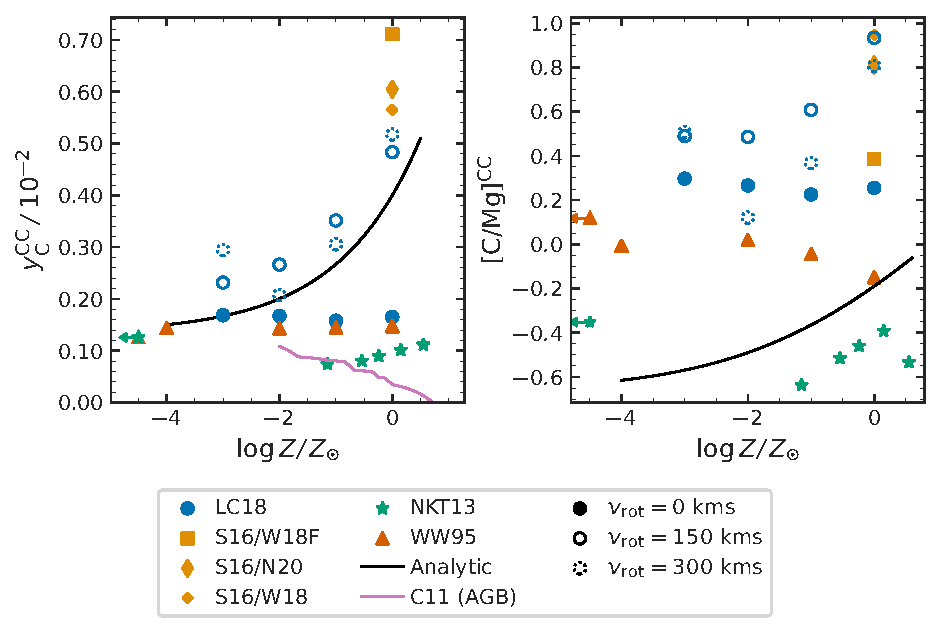
\includegraphics{cc_yields.pdf}
    \caption[]{
        C yields from high-mass stars.
        \textbf{Left} The IMF-weighted \cc\ yield of C as a function of metallicity.
        \textbf{Right} The \cc\ [C/Mg] abundance ratio, defined in Eq.~\ref{eq:c_mg_cc}. The black line is the derived C yield from section \ref{sec:equilibrium} and Eq.~\ref{eq:zeta}. Yields are shown for tables from 
    \citet[red triangles]{WW95}, \citet[orange squares and diamonds]{sukhbold+16}, 
    \citet[green stars]{NKT13}, and \citet[blue circles]{LC18}. \citet{sukhbold+16} report yields for different black hole landscapes, while \citet{LC18} provide yields at different rotational velocities.
    In the top panel, the pink line denotes $\Ycagb$ from \cxi{} for comparison. All models include wind yields. 
}
    \label{fig:y_cc}
\end{figure*}



\subsection{Equilibrium Abundances}\label{sec:equilibrium}

Building on \citepos{WAF17} analytic models of chemical equilibrium,
\citet{james+23} demonstrate that the relationship between N and O can be
explained by the metallicity dependence of their relative yields (see discussion
in their section 4.6).
We find similar results extending these arguments to C and Mg.
The equilibrium C/Mg abundance ratio is 
\begin{equation}\label{eq:equilibrium_yields}
    {\rm [C/Mg]_{eq}} = \log \left(\frac{\Ycc + \Ycagb }{y_{\rm Mg}}\right) - \log \left(\frac{Z_{\rm C,\,\odot}}{Z_{\rm Mg,\,\odot}}\right)
\end{equation}


We isolate the low-$\alpha$ sequence of subgiants to represent the equilibrium abundance trends, defined by [Mg/Fe] - [Fe/H] as in \citet{weinberg+19}.
Low-$\alpha$ stars are defined as stars with
\begin{equation}\label{eq:high_alpha}
\begin{cases}
\text{[Mg/Fe]} <0.12-0.13\,\text{[Fe/H]}, & \text{[Fe/H]}<0\\
\text{[Mg/Fe]} <0.12, & \text{[Fe/H]}>0. \\
\end{cases}
\end{equation}
with high-$\alpha$ stars being otherwise from \citet{weinberg+19, weinberg+22, emily+19, emily+21}.


In Fig.~\ref{fig:analytic}, we show the inferred C/Mg yield ratio against metallicity. 
\begin{subequations}\label{eq:yc_inferred}
    \begin{align}
        \frac{\Yct(Z)}{y_{\rm Mg}} &\approx 4.20 + 1.64 \log (Z/\Zo)\\
        \frac{\Yct(Z)}{y_{\rm Mg}} &\approx 4.12 + 1.21 \log(Z/\Zo) + 3.07 \log(Z/\Zo)^2
    \end{align}
\end{subequations}
These yield ratios results in an equilibrium abundance $[{\rm C/Mg}] = -0.09$ at solar metallicity, which is consistent with our subgiant sample and is within \about{20\%} of the solar C/Mg mixture. (check this!)



With the total C yield of Eq.~\ref{eq:yc_inferred} and given an \agb\ C yield, we can derive an \cc\ C yield that would predict observationally consistant [C/Mg] ratios.
\begin{subequations}
    \begin{align}
        \Ycc(\Zo) &= \Yct(\Zo) - \Ycagb(\Zo)\\
        \zeta^{\rm cc} &= \zeta - \zeta^{\rm agb}
    \end{align}
\end{subequations}
where $\zeta$ is the (solar) metallicity dependence of the C yield at $Z=\Zo$
\begin{equation}
    \zeta = \frac{d y_{\rm C}}{d Z} \Big \vert_{(Z=\Zo)},
\end{equation}
and $\zeta^{\rm cc}$ and $\zeta^{\rm agb}$ correspond to the specific enrichment channels. 
This method reduces the number of free parameters and enables all yield models to match \caah\ trends in \apogee{} subgiants, even when considering alternative \agb\ yield tables.
Table~\ref{tab:agb} provides $\zeta^{\rm agb}$ for each \agb\ yield table we consider.


Both observational and theoretical uncertainties limit the accuracy of our relative yield predictions.
Additionally, the derived yields will be systematically biased if the galaxy is out of equilibrium, e.g. due to a recent starburst \citep{mor+19,isern19}. 

\begin{figure}
    \centering
    \includegraphics{figures/equilibrium_yields.pdf}
    \caption[]{Inferred total C yields as a function of metallicity. We assume chemical equilibrium (orange curve, see discussion in section \ref{sec:equilibrium}). Blue points are the median value of $\Ycc$ for each (number) bin in [Mg/H] with uncertainties based on the 16--84 percentile range.
    }
    \label{fig:analytic}
\end{figure}



\subsection{Single-zone models and \caafe{}}
\dbnote{This will be a section I will write after a little more investigation. I think this should go by the equilibrium model, but maybe move both sections to after a discussion of the fiducial model: Multizone description $\to$ justify equilibrium and singlezone $\to$ consideration of other parameters. Or maybe just a different section?}


\section{The Multi-zone Model}\label{sec:vice}

Our models extends the \citet[hereafter \JJ]{james+21} Milky Way model, run with the publicly available Versatile Integrator for Chemical Evolution (\VICE).%
    \footnote{\VICE~is available at \url{https://github.com/giganano/VICE}}
This model is described extensively in \JJ~and concisely summarized  in \citet{james+23}. Here, we provide a brief overview of the relevant model components.

Classical, \textit{one-zone} models of chemical evolution assume instantaneous mixing of metals in the star-forming ISM\ \citep[e.g.][]{matteucci21}. This simple framework is a poor approximation of the Milky Way.  The Galaxy evolves \textit{inside-out} -- where star formation is higher towards the center and in the early universe \citep{WF91, kauffmann96, bird+13}. Stars can also migrate several kpc over their lifetimes, mixing different chemical environments across the galaxy \citep{bird+12,sellwood+binney02}. Multi-zone models account for stellar migration and changing environments by stitching together multiple one-zone models and mixing stellar populations. 

The Galaxy is divided into 200 rings, each representing a single, 100\,pc zone. Each ring (or zone) has a separate stellar population and gas supply. We initially assume an inside-out SFH from \JJ, where the star formation surface density $\dot{\Sigma}_\star$ is given by 
\begin{equation}\label{eq:inside_out}
    \dot{\Sigma}_\star \propto \left(1-e^{-t/\tau_{\rm rise}}\right) e^{-t/\tau_{\rm sfh}}.
\end{equation}
$\tau_\text{rise}=2$\,Gyr loosely describes when the star formation rate reaches a maximum, and $\tau_{\rm sfh}$ describes the decay timescale of star formation as a function of radius $R$. \JJ\ derive $\tau_{\rm sfh}(R)$ through analysis of four integral field spectroscopy surveys in \cite{sanches20}. At each $R$, the SFH is normalized to match the stellar surface density gradient \citep{BHG16} assuming a total stellar mass of $5.17\times10^{10}\,\Mo$ \citep{LM15}. Star formation ends beyond a radius $R=15.5\,$kpc, but stellar populations are allowed to migrate as far as $R=20\,$kpc.  
The gas inflow is calculated to maintain the SFH for each radius and time, using an extension of the Kennicutt-Schmidt law \citep{kennicutt98} motivated by the combined observations of \citet{bigiel+10} and \citet{leroy+13}, 
\begin{equation}
\dot{\Sigma}_{\star} \propto 
\begin{cases}
    {\Sigma}_{\rm gas} & 2\times 10^7 \Mo\,{\rm kpc}^{-2} \leq \Sigma_{\rm gas} \\ 
    {(\Sigma}_{\rm gas})^{3.6} & 5\times 10^6 \Mo\,{\rm kpc}^{-2}\leq \Sigma_{\rm gas} < 2\times10^7 \Mo\,{\rm kpc}^{-2}\\ 
    {(\Sigma}_{\rm gas})^{1.7} & \Sigma_{\rm gas} < 5\times10^6 \Mo\,{\rm kpc}^{-2}.
\end{cases}
\end{equation} 
The scaling of this relationship varies with time due to the redshift dependence of $\tau_\star$ in molecular gas observed by \citet{tacconi18}. We assume a \citet{kroupa01} IMF.


To account for radial migration, we use a normally-distributed, $\sqrt{\rm time}$ migration scheme. The final position of each star particle is sampled from
\begin{subequations}
\begin{align}
        R_{\rm end} &\sim N(R_{\rm birth}, \sigma_R ) \\
        \sigma_{R} &= 1.27\,{\rm kpc} \sqrt{\frac{t_{\rm end} - t_{\rm birth}}{\rm Gyr}}
\end{align}
\end{subequations}
At the boundaries, stars at $R=0$ move to $R=0$ if $R_{\rm end}<0$ and stars will move to $R=20$\,kpc if $R_{\rm end} > 20$\,kpc. \dbnote{would be better to change s.t. star truncates at 20 but moves there earlier...}
The star moves from its birth radius to its final radius via
\begin{equation}
        R(t) = \Delta R \sqrt{\frac{t - t_{\rm birth}}{t_{\rm end} - t_{\rm birth}}}
\end{equation}
The $\Delta R \propto \sqrt{\rm time}$ dependence arises when migration proceeds as a consequence of the diffusion of angular momentum \citep{frankel18, frankel20}.
At each time step, each star particle travels a radial distance sampled from 
where $N(\mu, \sigma)$ represents a draw from normal distribution and $dt=20$\,Myr is the simulation timestep.%
\footnote{Not shown here, we also explored variations of temporal, spatial resolution and migration strength and found these do not affect median trends significantly.}
We do not account for radial gas flows.
Not shown here, we also explore migration based on random walks and the \texttt{h277} hydrodynamical
simulation results (with simulation parameters as in \citealt{bird+21}; see also \citealt{christensen12, zolotov12, loebman12, BZ14}), which leaves our qualitative conclusions unchanged. 
The full impact of the details of a galaxy's dynamical history on its chemical evolution is still unknown.

As the strength of outflows controls the resulting $\alpha$-element abundances, we extend \JJ and create a metallicity gradient by defining
\begin{equation}\label{eq:mass_loading}
\eta(R) = \frac{y_{\alpha}^{\rm cc}}{Z_{\alpha}(R)} -1 + r + \tau_{\star} / \tau_{\rm sfh} 
\end{equation}
where 
\begin{equation}
    \log Z(R) = \log Z_{\alpha,\ \odot} + 
    0.29 + 
    \begin{cases}
        -0.015(R-5) & R < 5 \\
        -0.09(R-5) & R \geq 5
    \end{cases}
\end{equation}
and we approximate $\tau_\star/\tau_{\rm sfh} \approx 0.3$ 
adapted from \citet{hayden+14}.
This choice of $\eta(R)$ results in a [$\alpha$/H] gradient consistent with Milky Way observations \citep[e.g.][]{hayden+14, weinberg+19, frinchaboy+13}.
If we change our assumed $y_{\rm Mg}$, the values of $\eta$ will change similarly to maintain the correct chemical trends.


\section{Results}\label{sec:results}

\subsection{Evolution of Carbon Abundances}

Fig.~\ref{fig:c_evo} shows evolutionary tracks for every zone of the fiducial model for [C/Mg] against [Mg/H] and [Mg/Fe].
\caah\ trend quickly reaches our equilibrium state in \about{5}\,Gyr. \caafe\ tracks continue to evolve due to the long tail in the DTD of \ia. 


The evolution of abundances in our fiducial model:
\begin{enumerate}
    \item[(1)] Star formation begins. Initially, \cc\ dominate enrichment. [C/Mg] evolves with yields set by $\Ycc/\Yoc$, resulting in increasing values with [Mg/H].  [Mg/H] quickly approaches its equilibrium value, but Fe remains low in comparison (in agreement with \citealt{WAF17}).
    \item[(2)]  A few hundred million years later,  delayed sources  enrich the ISM. \agb\ stars release C, raising [C/Mg], and \ia\ expel Fe, lowering Mg/Fe. 
    \item[(3)] Several billion years later, [C/Mg] plateaus as C also approaches equilibrium. [Mg/H] reaches equilibrium. [Fe/H] continues to incrase due to ongoing \ia\ from old stellar populations.
    \item[(4)] In the final few billion years, [C/Mg] decreases slightly due to declining \agb\ C yields. \caah\ trends shift only slightly, and [Mg/Fe] slowly and steadily decreases.

\end{enumerate}


This evolution is driven most dominantly by our chosen elemental yields, their
dependence on metallicity, and their DTDs.
As we will demonstrate in section 5.2 below, the slope of the [C/Mg]-[Mg/H] trend is
set by the relative contributions of CCSNe and AGB stars to the overall C abundance.
The positive metallicity dependence of massive star C yields outweighs the negative
dependence of AGB star yields, causing [C/Mg] to increase with [Mg/H].


\begin{figure*}
\centering
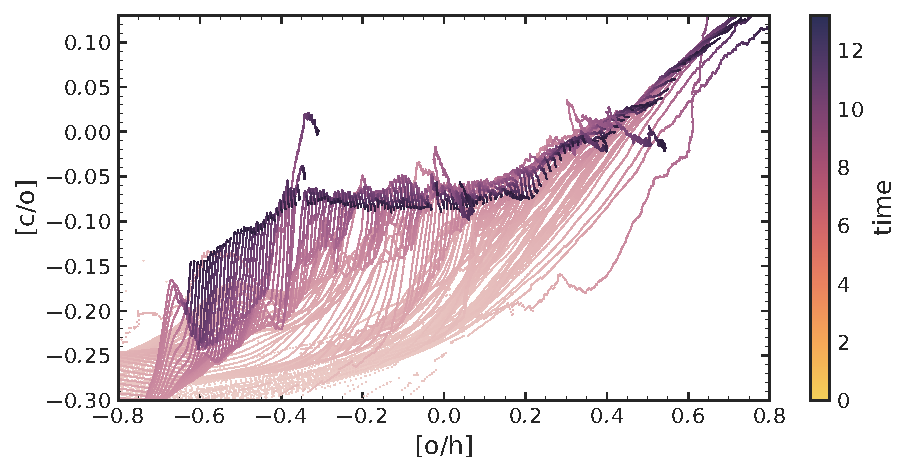
\includegraphics{figures/all_the_tracks.pdf}
\caption[]{
    Time evolution of gas-phase C abundances in our fiducial model.
    Each line represents a zone at a different galactic radii. The lines are colour-coded by time. The left shows \caah\ and the right \caafe. 
}
\label{fig:c_evo}
\end{figure*}



% note about \caafe plane
% As low-$\alpha$ stars were formed in regions closer to chemical equilibrium, we only plot the medians of the low-$\alpha$ sequences in \caah. 
% Instead, \caafe\ trends are set by the proportion of \agb\ C contribution. The \caafe{}-diagram, when restricted to a narrow range of metallicities, becomes an empirical delay-time-distribution of C. 
% High-$\alpha$ stars were formed in regions further from chemical equilibrium than stars with low [Mg/Fe]. Immediately after a star formation event, \cc\ elements dominate and only after sufficient time do \ia\ elements like Fe reach their higher-equilibrium abundances. 
% Likewise, high-[Mg/Fe] stars will have a greater portion of \cc\ C, as low-[Mg/Fe] stars will include more \agb\ C. 
% When binned in metallicity, median [C/Mg] changes by about 0.2 dex across the range of [Mg/Fe] at solar metallicities. As high-$\alpha$ stars have little to no delayed \ia\ Fe, these stars would also have little to no delayed \agb\ C. This means that AGB C stars make up about at most a fraction $f_{\rm agb} \approx 1 - 10^{-0.2} \approx 0.4$ of C production.
% 
% \begin{figure}
%     \centering
%     \includegraphics{apogee_caafe_binned.pdf}
%     \caption{Caption}
%     \label{fig:caafe_binned}
% \end{figure}

\subsection{Yield Variations}\label{sec:results_highmass}
\label{sec:agb_results}




\begin{figure*}
\includegraphics{sims_agb.pdf}

\caption[]{
    Stellar abundance trend predictions of our models . Coloured lines represent the median [C/Mg] in bins of [Mg/H] (left) or [Mg/Fe] (right) for each \agb\ table. Black points and grey dashes represent the median and 16th-84th percentiles of [C/Mg] in each bin in the \citetjack~sample. 
    The left panel only shows low-$\alpha$ stars. In the right panels, we show the trends only for stars where $-0.15\leq {\rm [Mg/H]}\leq -0.05$.
    Stars are binned into 20 (left) or 12 (right) equal number bins. 
}
\label{fig:first_models}
\end{figure*}


\begin{figure*}
\includegraphics{sims_zeta_f.pdf}

\caption[]{
    Similar to Fig.~\ref{fig:first_models}. 
    \textbf{Top}: Models with different metallicity dependences for  \cc\ C yields. \textbf{Bottom}: Different \agb\ fractinos of C.
}
\label{fig:zeta_f}
\end{figure*}


\begin{figure*}
\includegraphics{figures/sims_degens.pdf}

\caption[]{
    Similar to Fig.~\ref{fig:first_models}. 
    \textbf{Top}: Models with different metallicity dependences for  \cc\ C yields. \textbf{Bottom}: Different \agb\ fractinos of C.
}
\label{fig:sims_degens}
\end{figure*}




We evaluate our models by comparing predicted median stellar trends to our subgiant sample (see section~\ref{sec:data_selection}. 
We draw 12,000 stars from the simulated stellar populations such that the selection probability is proportional to a stellar population's mass and that the subsample follows the same distribution in Galactocentric radius as the subgiants. 


Fig.~\ref{fig:first_models} show the four C yield models (\cxi, \vxiii, \kxvi, \pxvi). For the most part, different \agb\ yield tables result in qualitatively similar predictions. \vxiii, however, does not reproduce solar trends as the model predicts strong C destruction at slightly super-solar metallicities, resulting in inversions in both \caah\ and \caafe. 
As all \agb\ models predict C yields to decline with metallicity, all models predict an increasingly downward slope in \caafe\ with [Mg/Fe]. A recent burst in star formation may hide this downturn (see section~\ref{sec:sfh}), but C destruction at the level predicted by \vxiii\ is not supported by our sample. 
Because the effects of alternate \agb\ yield sets are small, we focus on \cxi{} model for the remained of this paper. Alternate yield sets minimally affect our conclusions. 



The top of Fig.~\ref{fig:zeta_f} shows models with varying strengths of the $\Ycc$ metallicity dependence, $\zeta^{\rm cc}$. With higher $\zeta^{\rm cc}$, the model predicts a steeper \caah trend, owing to the direct relationship between the C/Mg equilibrium abundances and yield ratios. 
However, \caafe~is minimally affected by changes to $\zeta^{\rm cc}$ since \cc\ occurs on much shorter timescales than \ia\ and \agb\ enrichment.%
\footnote{The only effects on \caafe, when considering the narrow metallicity slice, are because of either the slight change in equilibrium abundances, the imperfect evolution of the galaxy, or that the ISM abundances are set by stars which were born at poorer metallicities. }
%  Hence, \caah\ tells us about the total C yield with metallicity, which \caafe\ is independent of. If we know the \agb\ C yields, then with observed \caafe\ abundance trends, we can infer the \cc\ C yields with metallicity.



The bottom of Fig.~\ref{fig:first_models} shows three models with different C \agb\  fractions, defined as 
\begin{equation}\label{eq:f_agb}
    f_{\rm agb} \equiv \frac{\Ycagb(\Zo)}{\Yct(\Zo)}.
\end{equation}
Modifications of $f_{\rm agb}$ affect \caafe{} trends significantly more than \caah. At fixed metallicity, the \caafe\ trend is principally sensitive to how much C and Fe comes from delayed sources. Increasing the \agb\ fraction therefore steepens the \caafe\ trend as expected. Though each yield model predicts the trend to flatten at ${\rm [Mg/Fe} \lesssim 0.1 $, the median is still within the width of the observed distribution and the overall agreement is good. 








\subsection{Variations in Star Formation History} \label{sec:sfh}

In this section, we consider an alternate SFH, namely one which exhibits a late-time elevation in the star formation rate. Motivated by the findings of \citet[see discussion in \JJ]{mor+19,isern19}, this \textit{lateburst} model
adds a Gaussian burst to the fiducial inside-out model, 
\begin{equation}\label{eq:lateburst}
    \dot{\Sigma}_\text{lateburst} \propto \dot{\Sigma}_\text{inside-out} \left(1 + A\,e^{-(t-\tau_{\rm burst})^2/2\sigma^2_{\rm burst}} \right)
\end{equation}
where $A=1.5$ represents the amplitude of the birth, $\tau_\text{burst}=10.8$\,Gyr is the time where the burst is strongest, and $\sigma_\text{burst}=1$\,Gyr is the width of the burst.
% Our earlyburst model is instead a double exponential, with the second exponential begining at $t_1=5\,$Gyr.
% \begin{equation}\label{eq:twoinfall}
%     \dot{\Sigma}_{\rm earlyburst} \propto A\,e^{-t/\tau_{\rm burst}} + 
% \begin{cases}
%     e^{-(t-t_1)/\tau_\text{sfh}} & t_1 < t \\
%       0 & t<t_1
% \end{cases}
% \end{equation}
% where we take the burst duration, $\tau_{\rm burst}=2$\,Gyr.
% This approximately corresponds to the Gaia-Encelidus merger, inducing higher star formation in the Milky Way \citep{spitoni21, bonaca20, helmi18}.

The bottom of Fig.~\ref{fig:first_models} compares the fiducial and lateburst models. The lateburst slightly shifts \caah\ down and only slightly perturbs \caafe. These variations are small compared to the width of the observed distribution. 
Building on \citet{james+23}, we therefore conclude that the \caah\ and \caafe\ trends reflect nucleosynthetic yields more than the Galactic SFH. 



\subsection{Degeneracies} \label{sec:outflows}

While some Milky Way \gce{} models (including ours) incorporate significant mass-loading, others
neglect mass-loading and instead use lower yields \citep[e.g.][]{MCM13, MCM14, spitoni19, spitoni20, spitoni21}.
Both classes of models are able to reproduce many details of the disk abundance structure due to the strong degeneracy between the normalizations of elemental yields and mass-loading (see discussion in, e.g. \citealt{sandford+22} and appendix B of \citealt{james+23}). 
Our parameterization of $\eta$ illustrates this (see Equation~\ref{eq:mass_loading}) -- choosing a lower value of $y_{\alpha}$ will similarly result in lower values of $\eta$ while maintaining the same metallicity gradient. 
We consider a model where we double all yields, in the top row of Fig.~\ref{fig:sims_degens}. A uniform change in yields and outflows leaves our median trends relatively unchanged. 

Additionally, Fe yields and the \ia\  delay-time-distribution have their own uncertainties. Increasing both $y_{\rm Fe}^{\rm Ia}$ and $\Ycagb$ correspondingly leaves \caafe\ mostly unchanged. 

Fig.~\ref{fig:sims_degens} demonstrates this point with a model in which we increase the \ia\ Fe yields by 20\% and increase $f_{\rm AGB}$ to 0.3. 
Fundamentally, the \caafe\ trends demand yield models in which these delayed components of C and Fe enrichment are in a particular proportion.

Finally, the delay-time-distribution of \agb\ stars is determined by the mass dependence of the yield. If we shift the yield tables down in mass artificially, then the delay-time-distribution of \agb\ C is more extended. A lower $f_{\rm agb}$ is needed to produce a similar trend in \caafe{}. The top panel of Fig.~\ref{fig:nitrogen} demonstrates this point with a model. 
Conversely, shifting the yield tables up in mass shortens the DTD and requires a higher \agb\ fraction in order to make up the difference (verify). 

Initial mass function (and possible metallicity dependence)? Metallicity dependent Oxygen/Magnesium and Iron yields? Gas phase migration?


\subsection{Nitrogen}


\begin{figure*}
\centering
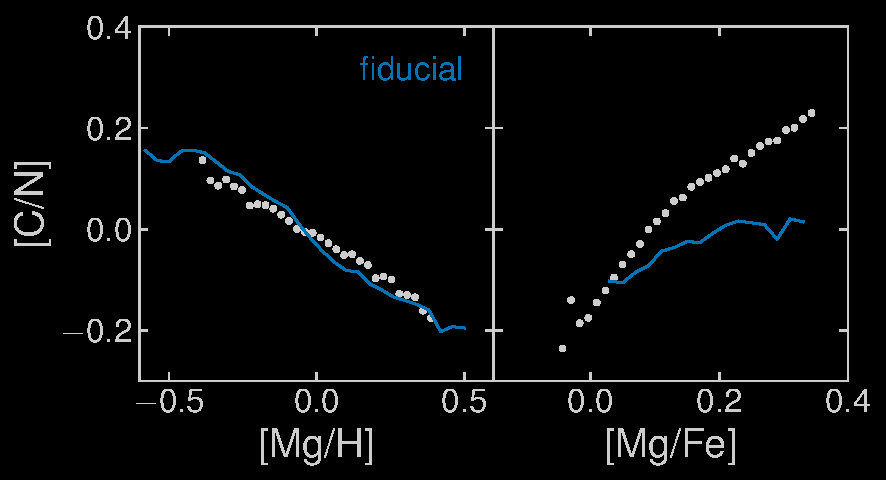
\includegraphics{figures/c_n.pdf}

\caption[]{Similar to Fig.~\ref{fig:first_models}. The top panels show models with different mass-ranges contributing \agb\ C yields. The middle panels show different star formation histories (section \ref{sec:sfh}) and yield normalizations. The bottom panels show [N/Mg] against [Mg/H] and [Mg/Fe] for the fiducial model.
}
\label{fig:nitrogen}
\end{figure*}

N production, also affected by the CNO cycle, is closely tied to C. As a test of our model, we use the \agb\ N yield suggested by \citet{james+23}.The bottom row of Fig.~\ref{fig:nitrogen} shows [C/N] versus [Mg/H] and [Mg/Fe] for our fiducial model. We are able to closely match the [N/Mg]-[Mg/H] trend. The [N/Mg]-[Mg/Fe] is predicted to be more shallow than observed -- a limitation of the model potentially implying a more extended DTD for N production. We do not explore this further here since our focus is C. 


Though photospheric abundances of both C and N in red giants are affected by FDU, (see discussion in section~\ref{sec:data_selection}), their total abundance is conserved by the CNO cycle [e.g. CITE]. C+N therefoe enables an additional test of the yields emperically calibrated in this paper and by \citet{james+23}. Thanks to the higher luminosities of red giants, we can make this comparison across a broader range of Galactocentric radii and, consequently, metallicity.

Fig.~\ref{fig:cn} shows the predicted [C+N/Mg]-[Mg/H] trend in comparison to \citepos{weinberg+22} sample, also taken from \apogee\ DR17 (see their section 3). The model predicts a slightly shallower trend than the data, though the differences are within the width of the observed distribution, with differences at the $<0.05$dex level at fixed [Mg/H]. 
While the number of stars in our subgiant sample drops off significantly at $\rm [Mg/H] \approx -0.3$, this comparison supports our empirically calibrated C and N yields down to $\rm [Mg/H] \approx-0.5$ (50\% lower in Z).



\section{Gas-Phase Abundances}\label{sec:gas}

\begin{table}
	\centering
    \caption[]{Single zone model parameters}
	\label{tab:singlezone_params}

	\begin{tabular}{l l l l l}
		\hline
        Model & $\eta$ & $t_{\rm end}$ & $\tau_\star$ & $\tau_{\rm sfh}$ \\
		\hline
        1 & 0 & 13 & 2 & 5\\
        2 & 1 & 10 & 2 & 10\\
        3 & 9 & 3 & 5 & 3\\
        4 & 12 & 2 & 10 & 2\\
		\hline
	\end{tabular}
\end{table}

As a final test of our model, we compare the predictions against C abundances
in the gas-phase.
These measurements are challenging since C lacks strong collisional excitation
lines, and its recombination lines fall in the ultraviolet with no nearby
H lines to reference~\citep[e.g.,][]{skillman+20}.
These two classes of spectral lines are also systematically discrepant at the
factor of~$\sim$2 level~\citep{GR07}.
As a consequence, the uncertainties associated with any one measurement are
substantial (see the representative error bars in Fig. 13), but we are able to
illuminate the underlying mean trends by combining observations from multiple
sources.
\par
Fig. 13 shows our compilation alongside the gas-phase abundances in our model
at snapshots of~$t = 2$ Gyr and the present day.
While we used Mg as our representative alpha element in our APOGEE sample, O
is more readily observed in the gas-phase, so we shift focus to C/O in this
section.
The model at the present day is consistent with the mean trend seen in HII
regions in the MW and similar star forming galaxies at redshift~$z \sim 0$.
Together with our results in~\S~5, this agreement suggests that our yield model
is an accurate description of C nucleosynthesis at metallicities typical of
MW-like galaxies.

Nonetheless, our model does not extend as low in metallicity as dwarf galaxies
or (especially) damped Lyman-alpha systems.
To test our model at these abundances, we run a suite of one-zone GCE models
with a handful of different parameter choices.
\note{[Describe parameter choices here, beginning with some fiducial set of
choices] Note: after seeing Fig. 13, I'd say it's worth using different
linestyles to mark the different parameter choices in Fig. 8 -- I'd stick
with black as color already differentiates between multi-ring and one-zone
models.}
Fig.~\ref{fig:gas_phase} also plots a single-zone model and time-slices of the fiducial multi-zone models gas-phase at present day and $t=2$\,Gyr. 
Our single-zone model is designed to have parameters broadly consistent with the Gaia-Encelidus sausage.
We evolve the singlezone model for 2\,Gyr, using mass loading $\eta=20$, star formation efficiency $\tau_{\star}=30\,{\rm Gyr}$, and a star formation history $\propto e^{-t/3{\rm\,Gyr}}$.
The single-zone model uses a 1.5 mass factor times f=0.25 C11 yields. Note that the mass shift results in significant C destruction by high-mass AGB stars at low metallicities, enabling the model to reproduce the low [C/O] abundances at [O/H] = -1.


\footnotetext{See e.g. CITATION. Th Gaia-Encelidus sausage (GSE) is a kinematically and chemically distinct group of halo stars consistant with the merger of a dwarf galaxy early in the Milky Way's formation.}

Each of these one-zone models predicts a steeper C/O-O/H trend than our
fiducial multi-ring model from previous sections.
This difference arises because the trend in the multi-ring models arises as a
superposition of end-points (see Fig. 7), qualitatively similar to, e.g.,
\citepos{schonrich-binney09} argument regarding
the low-alpha sequence.
In the one-zone models, the trend instead arises as an evolutionary sequence.
To demonstrate this point further empirically, Fig. 13 includes measurements
in halo and thick disk stars.
This sample indeed shows a C/O-O/H trend that is clearly steeper than our
fiducial multi-ring model, which is an accurate representation of the APOGEE
low-alpha sequence (see Fig. 8).

At the lowest metallicities ($\log_{10}(Z / Z_\odot) \lesssim -2$), our suite
of one-zone models is consistent with the C/O ratios seen in damped Lyman-alpha
systems.
For all parameter choices, these ratios simply reflect the relative C and O
yields of low-metallicity massive stars (see Fig. 5), with the increase in C/O
at higher metallicities arising due to the onset of AGB star enrichment (see
Fig. 7).
As a consequence, our yield model as parameterized predicts that C/O ratios
should never be significantly below~$\sim$half solar.
This prediction is challenged by the measurements in both dwarf galaxies and
halo/thick disk stars in Fig. 13, which suggest ratios~$\sim$$0.2 - 0.3$ dex
below solar between~$\log$(O/H) = X and Y.

This discrepancy could arise at least in part due to failures of our yield
prescription and, by extension, could point to shortcomings in stellar
nucleosynthesis models.
However, we cannot rule out the possibility of systematic uncertainties in
abundance determinations playing a role.
At these metallicities, deviations from local thermal equilibrium (LTE) can
bias measurements at the~$\sim$0.2 dex level~\citep[e.g.,][]{amarsi+19}.
Considerations of non-LTE effects are not included in our APOGEE sample, but
the corrections are smaller near solar metallicity.

\begin{figure*}
\centering
\includegraphics[]{figures/summary_plot.pdf}
\caption[]{Gas-phase C abundances. We plot our model at $t=2$\,Gyr and present day as thick solid lines. Black lines are single-zone models. Points represent measurements in 
    HII regions    \citep[pink circles;][]{skillman+20, esteban+02, esteban+09, esteban+14, esteban+19}
    damped Lyman-alpha (DLA) systems \citep[blue triangles;][]{ellison+10, srianand+10, dutta+14, DZ+03, pettini+08, morrison+16,cooke+17},  % a1: Cooke et al. (2015); 2: Dutta et al. (2014); 3: Cooke et al. (2014); 4: Ellison et al. (2010); 5: Cooke et al. (2011b); 6: This work; 7: Pettini et al. (2008); 8: Morrison et al. (2016); 9: Srianand et al. (2010); 10: Cooke et al. (2012); 11: Dessauges-Zavadsky et al. (2003)
    dwarf galaxies \citep[red diamonds;][]{berg+19},
    Milky Way halo and thick disk stars \citep[green stars;][]{amarsi+19, nissen+14, fabbian+09},
    and Milky Way high-$\alpha$ stars (yellow points; \citealtjack), and high redshift galaxy through JWST \citep[yellow hexagon;][]{arellano-cordova+2022}.
}

\label{fig:gas_phase}
\end{figure*}


\section{Conclusions}\label{sec:conclusions}


Building on~\citet{james+23}, we quantify the impact of C yield assumptions on Milky Way GCE models. We use Roberts et al.'s (2023) sample of APOGEE subgiants as our primary observational benchmark, as subgiant atmospheres most likely reflect their birth C abundances (see discussion in section~\ref{sec:data_selection}).
In our fiducial model, C initially increases following the slope of the \cc\ C dependence. Later, AGB contributions from C cause a sharp rise in \caah, which slows down due to declining AGB C production and the approach towards equilibrium. The chemical elemental reach a quasi-equilibrium within \about{5}\,Gyr. As a result, the current C/Mg versus metallicity gradient is a superposition of equilibrium states, mixed together from different Galactic positions.


The slope of the predicted \caah\ relation is principally sensitive to the collective metallicity dependence of \cc\ C yields.
While AGB yields are predicted to decline with metallicity, out models show that \cc\ dominate the trend and make an overall positive metallicity trend. 
As the strength of the \cc\ metallicity dependence increases, the slope of the \caah\ trend correspondingly increases. The small effects of \agb\ C yield on the \caah\ trend can be easily corrected by small adjustments of the \cc\ yield's metallicity dependence.
Our predicted slope of NUMBER is approximately consistent with the \citet{LC18} rotating stellar models, however no simulation contains sufficient mass resolution or accuracy to reproduce the observed trends accurately. 

Because massive star enrichment dominates the C mass budget in our models, the predictions are relatively insensitive to the choice of AGB star yield model.
Of the \agb\ tables tested here, \cxi, \kxvi, and \pxvi\ all predict similar abundance trends in [C/Mg] with [Mg/H] and [Fe/Mg]. The strong destruction of C by massive stars at \about{} solar metallicity   in \vxiii\ are instead in tension with the data (See Figs.~\ref{fig:first_models})  and~\ref{fig:agb-ssp})
As both the \cxi\ and \pxvi\ models predict \about{} linear N yields as well, these combined models best explain combined C and N abundance trends (see Appendix!?).

As in~\citet{james+23}, we have constrained yield ratios as opposed to absolute yields. For example, scaling yields and outflows by a corresponding factor leaves abundance ratio trends unchanged (Fig.~\ref{fig:sims_degens}).  Effects such as black hole formation could create systematic shifts on predicted chemical yields.
Variations in the SFH instead only induce minor systematic shifts


When combined with~\citeauthor{james+23}'s~\citeyearpar{james+23} empirically calibrated N yields, we find that our fiducial model accurately describes the [C/N]-[Mg/H] relation in our sample. The [C/N]-[Mg/Fe] relation, on the other hand, is shallower than the data, indicating that the DTD of C production may be sharper than our AGB yield tables would suggest (or the N DTD more extended, or both).

Finally, we compare our models againsts a compilation of literature gas-phase and halo-star abundances (see Fig.~\ref{fig:gas_phase}). Our fiducial model fails to explain the lowest values of [C/O] at metallicities of -1 to -2. We briefly consider a modified variation of the CCSNe yield of C which drops to explain these values, which maintains trends consistant with APOGEE. 


Our results demonstrate the power of empirically calibrated stellar yields. In our GCE models, trends in abundance ratios with metallicity are largely determined by trends in yield ratios with metallicity. As a result, the metallicity dependence of the total, population-averaged C yield is tightly constrained by the [C/Mg]-[Mg/H] relation, but the metallicity dependencies of the individual contributions from CCSNe and AGB stars are less precisely determined. Due to the sensitivity of elemental yields to poorly understood processes, such as mass-loss rates and convection, our results provide a useful benchmark for stellar evolution models~\citep[see the discussion in e.g.][]{gil-pons2022}. With abundance measurements for several million stars provided by upcoming spectroscopic surveys, particularly SDSS-V's Milky Way Mapper program~\citep{sdssv}, constraints on both stellar nucleosynthesis and the assembly history of our Galaxy will become increasingly more powerful.

More C observations across different galactic environments will continue to refine a complete understanding of C production, including the yields of the first stars,  evolution in the bulge, and so on. 


\section*{Acknowledgements}

 Here you can thank helpful
colleagues, acknowledge funding agencies, telescopes and facilities used etc.
Try to keep it short.

Software that has contributed to this work included  
\VICE~\citep{JW20, james+21},
\textsc{matplotlib} \citep{matplotlib},
\textsc{scipy} \citep{scipy},
\textsc{IPython} \citep{ipy},
\textsc{pandas} \citep{pandas},
\textsc{numpy} \citep{numpy},
\textsc{astropy} \citep{astropy:2013, astropy:2018, astropy:2022},
and 
\textsc{seaborn} \citep{seaborn}
.
Additionally, we thank \citet{OhioSupercomputerCenter1987} for the use of its facilities for the simulations. 

\apogee\ is part of SDSS-IV \citep{sloan_telescope, apogee_instrumentation, sdss_iv_overview, sdss17, apogee17, aspcap}.

Funding for the Sloan Digital Sky 
Survey IV has been provided by the 
Alfred P. Sloan Foundation, the U.S. 
Department of Energy Office of 
Science, and the Participating 
Institutions. 

SDSS-IV acknowledges support and 
resources from the Center for High 
Performance Computing  at the 
University of Utah. The SDSS 
website is www.sdss4.org.

SDSS-IV is managed by the 
Astrophysical Research Consortium 
for the Participating Institutions 
of the SDSS Collaboration including 
the Brazilian Participation Group, 
the Carnegie Institution for Science, 
Carnegie Mellon University, Center for 
Astrophysics | Harvard \& 
Smithsonian, the Chilean Participation 
Group, the French Participation Group, 
Instituto de Astrof\'isica de 
Canarias, The Johns Hopkins 
University, Kavli Institute for the 
Physics and Mathematics of the 
Universe (IPMU) / University of 
Tokyo, the Korean Participation Group, 
Lawrence Berkeley National Laboratory, 
Leibniz Institut f\"ur Astrophysik 
Potsdam (AIP),  Max-Planck-Institut 
f\"ur Astronomie (MPIA Heidelberg), 
Max-Planck-Institut f\"ur 
Astrophysik (MPA Garching), 
Max-Planck-Institut f\"ur 
Extraterrestrische Physik (MPE), 
National Astronomical Observatories of 
China, New Mexico State University, 
New York University, University of 
Notre Dame, Observat\'ario 
Nacional / MCTI, The Ohio State 
University, Pennsylvania State 
University, Shanghai 
Astronomical Observatory, United 
Kingdom Participation Group, 
Universidad Nacional Aut\'onoma 
de M\'exico, University of Arizona, 
University of Colorado Boulder, 
University of Oxford, University of 
Portsmouth, University of Utah, 
University of Virginia, University 
of Washington, University of 
Wisconsin, Vanderbilt University, 
and Yale University.



%%%%%%%%%%%%%%%%%%%%%%%%%%%%%%%%%%%%%%%%%%%%%%%%%%
\section*{Data Availability}

 
The inclusion of a Data Availability Statement is a requirement for articles published in MNRAS. Data Availability Statements provide a standardised format for readers to understand the availability of data underlying the research results described in the article. The statement may refer to original data generated in the course of the study or to third-party data analysed in the article. The statement should describe and provide means of access, where possible, by linking to the data or providing the required accession numbers for the relevant databases or DOIs.


%%%%%%%%%%%%%%%%%%%% REFERENCES %%%%%%%%%%%%%%%%%%
\bibliographystyle{mnras}
\bibliography{main}


%%%%%%%%%%%%%%%%% APPENDICES %%%%%%%%%%%%%%%%%%%%%

\appendix


\section{Comparison with other samples}

Discuss
\begin{description}
    \item \citet{vincenzo+21}
    \item Gaia-ESO survey
    \item \citet{bensby+21}
    \item \citet{weinberg+22}
    \item GALAH: Low completion, one line (6588Å), likely observational effects of lower detection rates for metal poor stars, but also strong systematic from APOGEE.
    \end{description}

    There are large spectroscopic surveys (RAVE, LAMOST)  but they do not have C abundances.

\begin{figure}
    \centering
    \includegraphics{c+n.pdf}
    \caption{[C+N/Mg]}
    \label{fig:cn}
\end{figure}

\begin{figure}
    \centering
    \includegraphics{figures/cmg_mgh_allstar.pdf}
    \includegraphics{figures/cmg_mgfe_allstar.pdf}
    \caption{Caption}
    \label{fig:enter-label}
\end{figure}

\bsp	% typesetting comment
\label{lastpage}
\end{document}




